\chapter{Mapping}
\label{chap:mapping}

\section{Existing implementations}
This chapter decribes the process of building a separate static and a dynamic map (containing non-moving and moving obstacles, respectively) based on radial distance measurements (in this case provided by a LIDAR). Isolating the static and the moving obstacles from each other has its difficulties but also its advantages. First of all, the implemented local track planner calculates safer, more optimized paths if it is informed of both the static and the dynamic obstacles along the path. Secondly, \href{https://en.wikipedia.org/wiki/Simultaneous_localization_and_mapping}{SLAM} (Simultaneous localization and mapping) algorithms work better if the their input contains only static objects in the space, because they build an internal map of the world. Passing detections of moving obstacles to a SLAM algorithm may lead to worse localization quality, as they may ruin this map.

As a first subtask of the mapping project, I checked if any implementation is avaiable already, that can handle dynamic objects. The only possible candidate was \href{http://wiki.ros.org/gmapping}{gmapping}, which is a popular ROS package, used in a wide variety of applications that require map-building and localization. Its SLAM algorithm takes LIDAR measurements as its input and generates an occupancy grid (a 2D map) of the car's environment. By using this map it is able to make corrections to the car's odometry-based position and orientation, which is usually inaccurate. I tried out the package, and the result maps were promising, the generated map was insensitive to the car's longitudinal movements and its rotations. But unfortunately, gmapping's SLAM does not support dynamic objects. See \ref{chap:static_map} for further details. Therefore, gmapping could not be used as the producer of the static map. But that didn't mean it couln't be used for its second feature, localization. Note, that the mapping implementation I made is not a SLAM algorithm, it is not able to make corrections to the car's pose. So for that purpose, I still needed the help of gmapping, which proved to be very reliable at localization. But the static map-building needed to be implemented internally.

\section{Method}
This chapter decribes the process of building a separate static and a dynamic map (containing non-moving and moving obstacles, respectively) based on radial distance measurements (in this case provided by a LIDAR). Isolating the static and the moving obstacles from each other has its difficulties but also its advantages. First of all, the implemented local track planner calculates safer, more optimized paths if it is informed of both the static and the dynamic obstacles along the path. Secondly, \href{https://en.wikipedia.org/wiki/Simultaneous_localization_and_mapping}{SLAM} (Simultaneous localization and mapping) algorithms work better if the their input contains only static objects in the space, because they build an internal map of the world. Passing detections of moving obstacles to a SLAM algorithm may lead to worse localization quality, as they may ruin this map.

As a first subtask of the mapping project, I checked if any implementation is avaiable already, that can handle dynamic objects. The only possible candidate was \href{http://wiki.ros.org/gmapping}{gmapping}, which is a popular ROS package, used in a wide variety of applications that require map-building and localization. Its SLAM algorithm takes LIDAR measurements as its input and generates an occupancy grid (a 2D map) of the car's environment. By using this map it is able to make corrections to the car's odometry-based position and orientation, which is usually inaccurate. I tried out the package, and the result maps were promising, the generated map was insensitive to the car's longitudinal movements and its rotations. But unfortunately, gmapping's SLAM does not support dynamic objects. See \ref{chap:static_map} for further details. Therefore, gmapping could not be used as the producer of the static map. But that didn't mean it couln't be used for its second feature, localization. Note, that the mapping implementation I made is not a SLAM algorithm, it is not able to make corrections to the car's pose. So for that purpose, I still needed the help of gmapping, which proved to be very reliable at localization. But the static map-building needed to be implemented internally.

In order to create two disjunct maps, one static and one dynamic, the key element of the process is the separation of the moving and non-moving obstacles of the measured points. After determining these two disjunct set of points, the maps can be converted to any desired or required format. Static maps are usually published as occupancy grids, while dynamic obstacles need to present information about their speed vector. Occupancy grids do not group the grid points according to their probabilities, therefore they do not know about the obstacles' borders and areas\footnote{In this project, 2D LIDARs were used, therefore the measured objects were seen as 2D shapes that have areas, not 3D objects that have volumes}. Dynamic obstacles however can be either represented as separate points with their own speed vectors, or groups of points, each groups having one speed vector. I chose the latter representation, thus publishing groups that contain a set of points (all the points, ideally) of the same obstacle. This way there is a one-to-one relationship between moving obstacles and groups. The separation and grouping methods of the mapping process is shown on diagram \ref{mapping_method}.

\tikzset{
     base_node/.style = {rectangle, rounded corners, draw=black,
                         minimum width=4.5cm, minimum height=1cm,
                         text centered, font=\sffamily},
  inout_node/.style   = {base_node, fill=blue!30},
  common_node/.style  = {base_node, fill=orange!15},
  dynamic_node/.style = {base_node, fill=green!30},
  static_node/.style  = {base_node, fill=red!30},
  decoration={brace},
  tuborg/.style={decorate},
  tubnode_left/.style={midway, left=2pt},
  tubnode_right/.style={midway, right=2pt}
}

\begin{figure}[!ht]
    \begin{tikzpicture}[
            node distance=1.5cm,
            every node/.style={fill=white, font=\sffamily}, align=center]
        % Input node
        \node (scan)            [inout_node]                                   {Input scan};
        % Common nodes
        \node (convert_abs)     [common_node, below of=scan]                   {Convert to absolute points};
        \node (dynamic_points)  [common_node, below of=convert_abs]            {Find dynamic points};
        \node (groups)          [common_node, below of=dynamic_points]         {Make dynamic groups};
        \node (separate)        [common_node, below of=groups]                 {Separate static points from groups};
        % Dynamic nodes
        \node (areas)           [dynamic_node, below of=separate, xshift=-3cm] {Measure areas};
        \node (tracking)        [dynamic_node, below of=areas]                 {Track groups};
        \node (publish_dynamic) [inout_node, below of=tracking]                {Publish dynamic obstacles};
        % Static nodes
        \node (update_map)      [static_node, below of=separate, xshift=3cm]   {Update static map};
        \node (publish_static)  [inout_node, below of=update_map]              {Publish static points};
        % Common connections
        \draw[->]           (scan) -- (convert_abs);
        \draw[->]    (convert_abs) -- (dynamic_points);
        \draw[->] (dynamic_points) -- (groups);
        \draw[->]         (groups) -- (separate);
        % Dynamic connections
        \draw[->]       (separate) -- (areas);
        \draw[->]          (areas) -- (tracking);
        \draw[->]       (tracking) -- (publish_dynamic);
        % Static connections
        \draw[->]       (separate) -- (update_map);
        \draw[->]     (update_map) -- (publish_static);
        % Decorations
        \draw[tuborg, decoration={brace}] let \p1=(scan.north), \p2=(separate.south) in
            ($(\x1+3.4cm, \y1)$) -- ($(\x1+3.4cm, \y2)$) node[tubnode_right] {Separation + grouping};
        \draw[tuborg, decoration={brace}] let \p1=(areas.north), \p2=(publish_dynamic.south) in
            ($(\x1-3cm, \y2)$) -- ($(\x1-3cm, \y1)$) node[tubnode_left] {Dynamic};
        \draw[tuborg, decoration={brace}] let \p1=(update_map.north), \p2=(publish_static.south) in
            ($(\x1+3cm, \y1)$) -- ($(\x1+3cm, \y2)$) node[tubnode_right] {Static};
    \end{tikzpicture}
    \caption{Mapping method}
    \label{mapping_method}
\end{figure}

The diagram consists of 3 subgraphs - these are also marked on the diagram. The first, and most important is the separation and grouping of dynamic points. The second subgraph describes the additional calculations that need to be done for the dynamic obstacles, and consists the documentation for the message structure definining these dynamic obstacles. And the third one is about the static map that is built from the static points. The sections under \ref{chap:mapping} explain these subgraphs in detail.

\begin{minipage}{\textwidth}
\section{Input parameters}
\label{chap:input_parameters}
The following input parameters can manipulate the mapping node:

\textbf{LIDAR\_MAX\_DIST} [meter]

The maximum measurable distance by the LIDAR(s). Depends on the LIDAR's characteristics.

\textbf{MAP\_RES} [meter]

The resolution of the built static map. Increasing this this value helps building a better quality map, but also increases the node's resource need.

\textbf{MAP\_SIZE} [meter]

The size of the built static map. Increasing this this value helps building a better quality map, but also increases the node's resource need.

\textbf{SINGLE\_LIDAR} [boolean]

Defines if the node's input is one LIDAR scan, or a separate front and rear scan that needs to be handled separately.
\end{minipage}

\section{Separation and grouping}
\label{chap:separation_and_grouping}
This section describes the method of separating dynamic and static points of the input scan. This step is essential in the pipeline of creating two disjunct maps.

\subsection{Input scan}
The input of the mapping algorithm is a 2D LIDAR scan, consisting of radial distance measurements. Two types of LIDARs were used in the project, \href{http://www.slamtec.com/en/lidar/a1}{RPLidar A1} and \href{http://www.slamtec.com/en/lidar/a2}{RPLidar A2}.
Both types have the following specifications:

\begin{center}
    \begin{tabular}{ | c | c | }
        \hline
        Scan rate           & 10 Hz            \\
        \hline
        Sample rate         & 8000 samples/sec \\
        \hline 
        Distance resolution & 0.2 centimeters  \\
        \hline 
        Angular resolution  & 1°               \\
        \hline 
        Detection range     & 12 meters        \\
        \hline
    \end{tabular}
\end{center}

The devices proved to be reliable, and for a project of this volume, their frequencies, resolutions and ranges were adequate. Their output is a ROS message of type \href{http://docs.ros.org/melodic/api/sensor_msgs/html/msg/LaserScan.html}{\textit{sensor\_msgs/LaserScan}}, which has the following structure:

\begin{minipage}{\textwidth}
\begin{lstlisting}[language=IDL]
std_msgs/Header header
float32 angle_min
float32 angle_max
float32 angle_increment
float32 time_increment
float32 scan_time
float32 range_min
float32 range_max
float32[] ranges
float32[] intensities
\end{lstlisting}
\end{minipage}

Among numerous other things, the message contains an array of radial distances (\textit{ranges}), that are the measurements themselves. The messages can be visualized easily using rviz.

\begin{figure}[!ht]
    \centering
    \subfloat[Gazebo simulation]
    {
        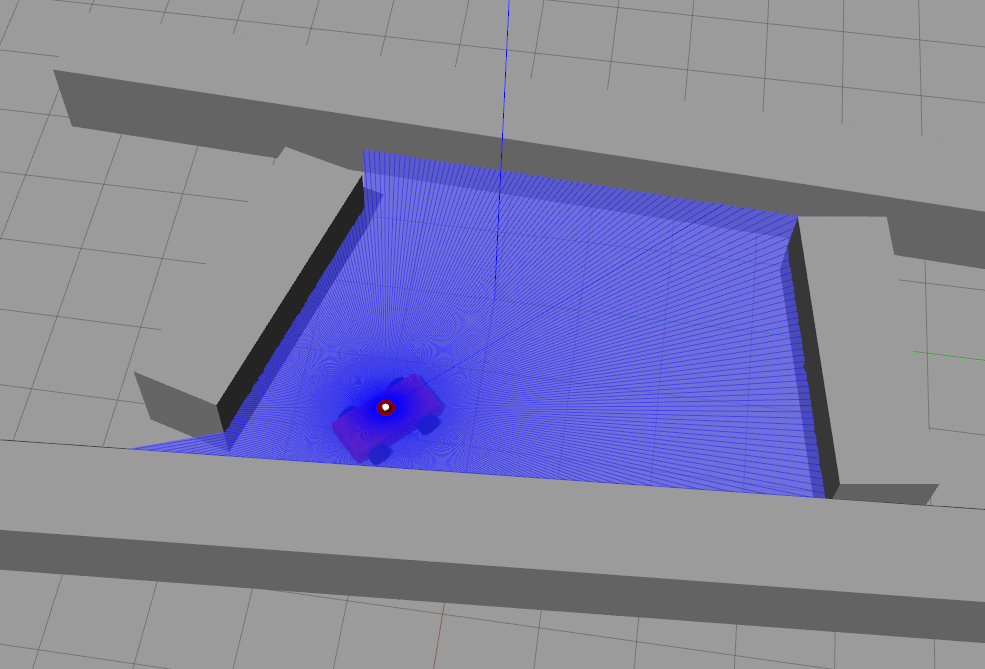
\includegraphics[height=48mm]{figures/raw/gazebo_lidar_scan.png}
        \label{gazebo_lidar_scan}
    }
    \subfloat[rviz visualization]
    {
    	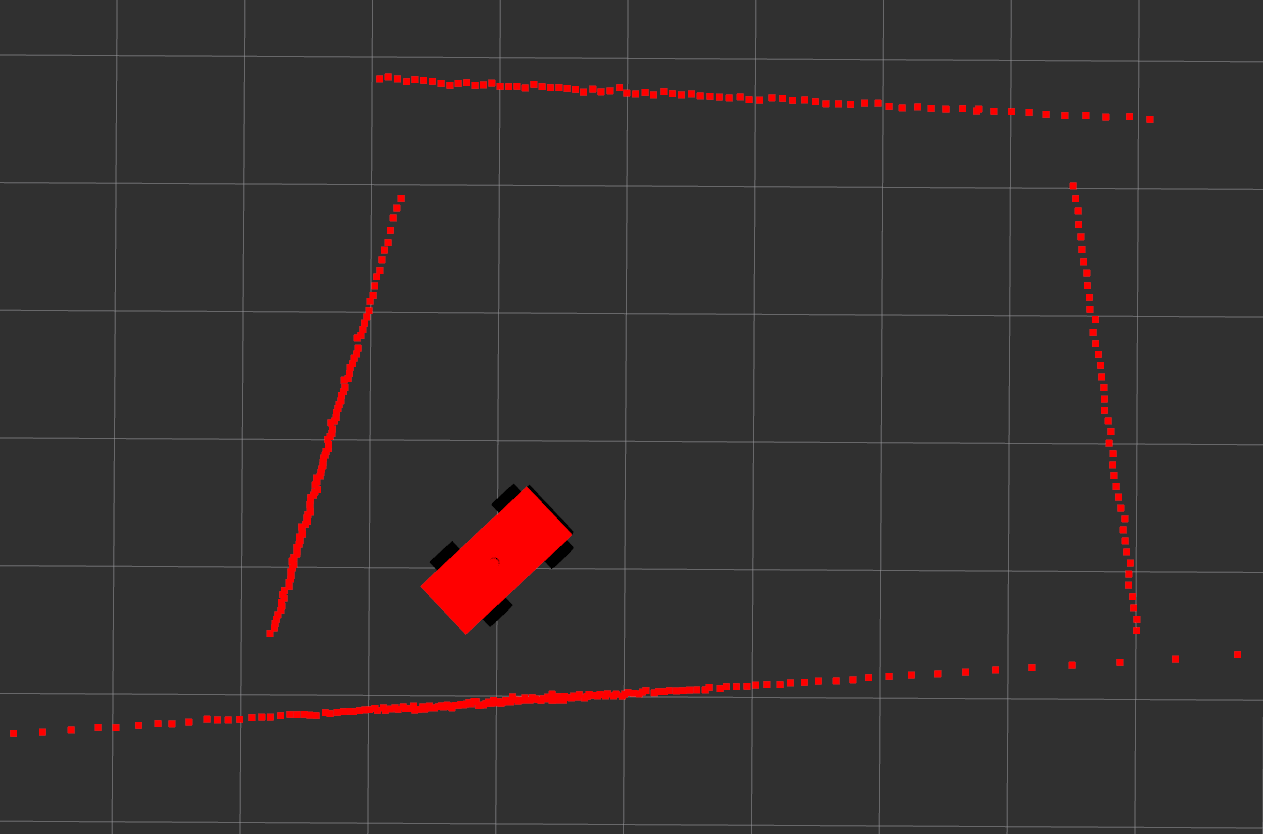
\includegraphics[height=48mm]{figures/raw/rviz_lidar_scan.png}
        \label{rviz_lidar_scan}
    }
    \caption{LIDAR scan}
    \label{lidar_scan}
\end{figure}

\subsection{Absolute points}
\label{chap:absolute_points}
For static map-building, absolute points\footnote{Absolute points are not relative to the car, but to a fix base point.} are needed in the space, and static-dynamic point separation also uses absolute points, so firstly, these radial distances need to be transformed. However, the internal static map and the static-dynamic separation use different coordinate systems. In order to understand the need for this, let's take a look at figure \ref{rqt_input}.

\begin{figure}[!ht]
    \centering
    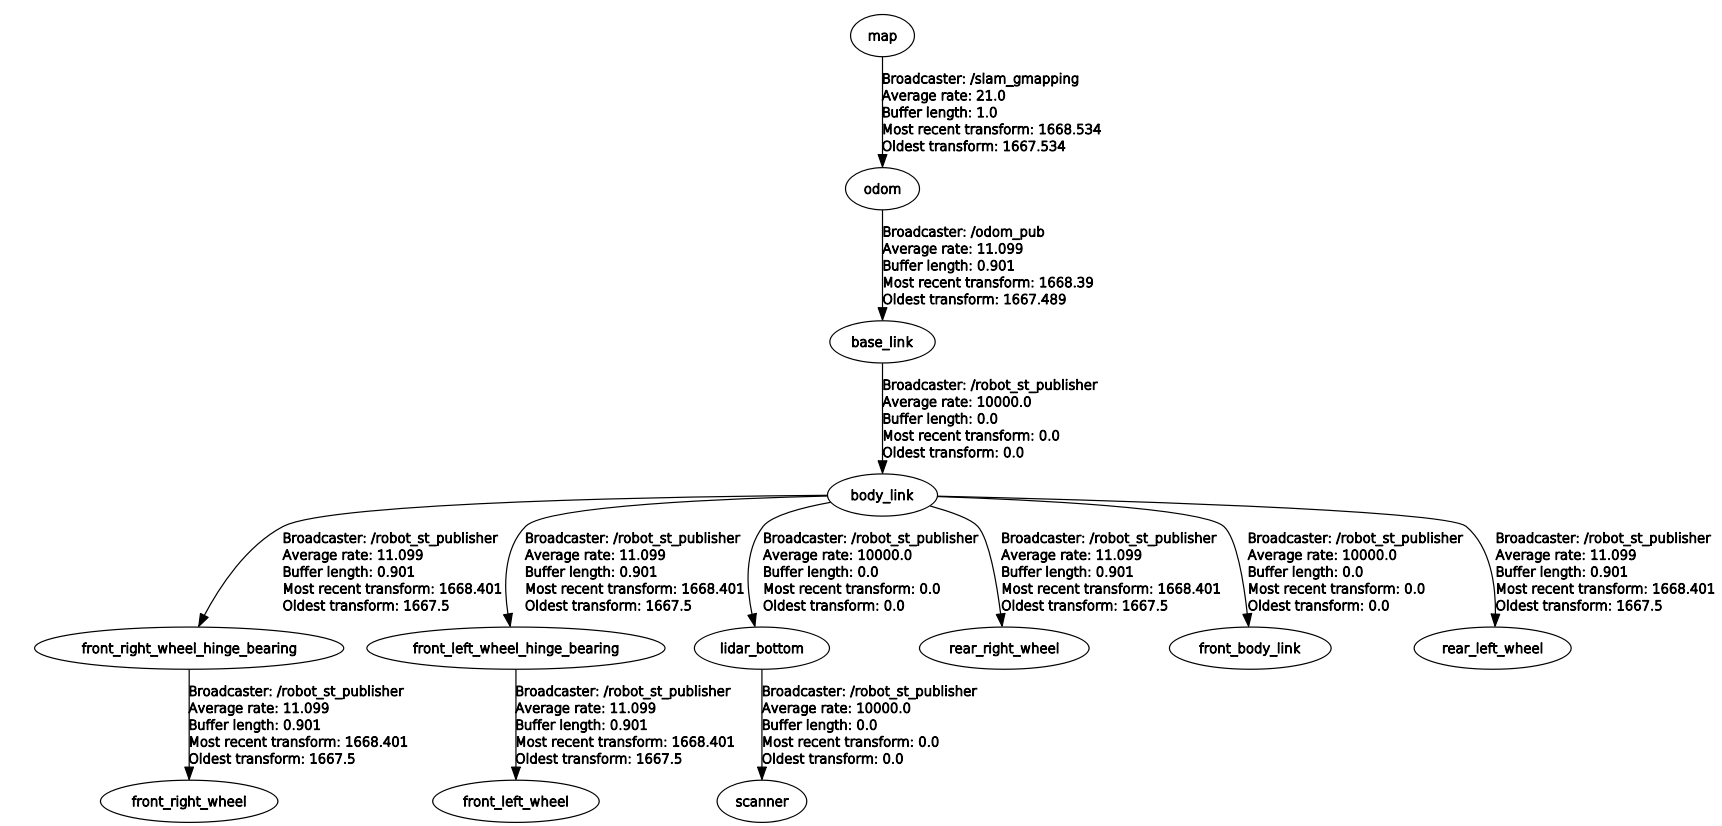
\includegraphics[height=130mm]{figures/raw/rqt_input.png}
    \caption{Coordinate frames}
    \label{rqt_input}
\end{figure}

As the figure shows, there are 3 coordinate frames that are important to the current case. The \textit{odom} frame is the car odometry's coordinate system. It is calculated from values measured on the vehicle, such as servo position and speed. The odometry is also published as a message of format (\href{http://docs.ros.org/melodic/api/nav_msgs/html/msg/Odometry.html}{\textit{nav\_msgs/Odometry}}), that has the following structure:

\begin{minipage}{\textwidth}
\begin{lstlisting}[language=IDL]
std_msgs/Header header
string child_frame_id
geometry_msgs/PoseWithCovariance pose
geometry_msgs/TwistWithCovariance twist
\end{lstlisting}
\end{minipage}

The message contains the car's position and orientation in \textit{pose} and its linear and angular speed in \textit{speed}.

The \textit{scanner} frame is the LIDAR's coordinate system. The transformation between \textit{odom} and \textit{scanner}\footnote{The implementation supports one and two LIDARs as well. In case of the two-LIDAR setup, instead of the \textit{front\_scanner} there is a \textit{rear\_scanner} and a \textit{scanner} frame.} is basically the pose of the LIDAR, relative to the car. The \textit{map} frame is the output of gmapping's localization. Basically, gmapping takes the car odometry and the LIDAR scans as its input, and corrects the odometry using SLAM. As a result the difference between frames \textit{map} and \textit{odom} will increase with time.

The internal static map in my implementation uses this corrected \textit{map} frame as the base for its points, so that its error is minimized. But unfortunately, the static-dynamic separation method cannot use this frame. The reason is that this frame does not get updated on every new scan, but with a much slower frequency. Therefore there are 'jumps' in the \textit{map} frame, which would cause false dynamic point detections (see \ref{chap:dynamic_points}). To avoid this undesired situation, the static-dynamic separation uses the \textit{odom} frame as its base, which is more continuous than the \textit{map} frame.

Therefore, two transformations are needed for each input point. The transformations are calculated using \href{http://wiki.ros.org/tf}{tf}, which maintains the relationship between coordinate frames in a tree structure (see figure \ref{rqt_input}) buffered in time, and makes the transformation of points, vectors, etc possible at any desired point in time.

\subsection{Dynamic points}
\label{chap:dynamic_points}
The next step is similar to a creating a subtraction image in image processing, where subtracting two images, taken from the same position but at a different time, results in an image that amplifies the movements between the snapshots. Previous methods\cite{RealTimeDynamicObjectDetection} that I studied before starting my implementation are also based on this step. The aim of this algorithm unit is basically the same: selecting the points from the input that are likely to be part of a moving mass. This is done by finding the points among the current measurements that have not been present in the previous ones.

This step is best explainable in practice. Let's assume that the position and orientation of the LIDAR is fix, and one object (e.g. a car) in the detected area is moving. Figure \ref{obstacle_movement} shows this situation. On the image, the pale contour represents the previous pose of the object, and the current state is blue.

\begin{figure}[!ht]
    \centering
    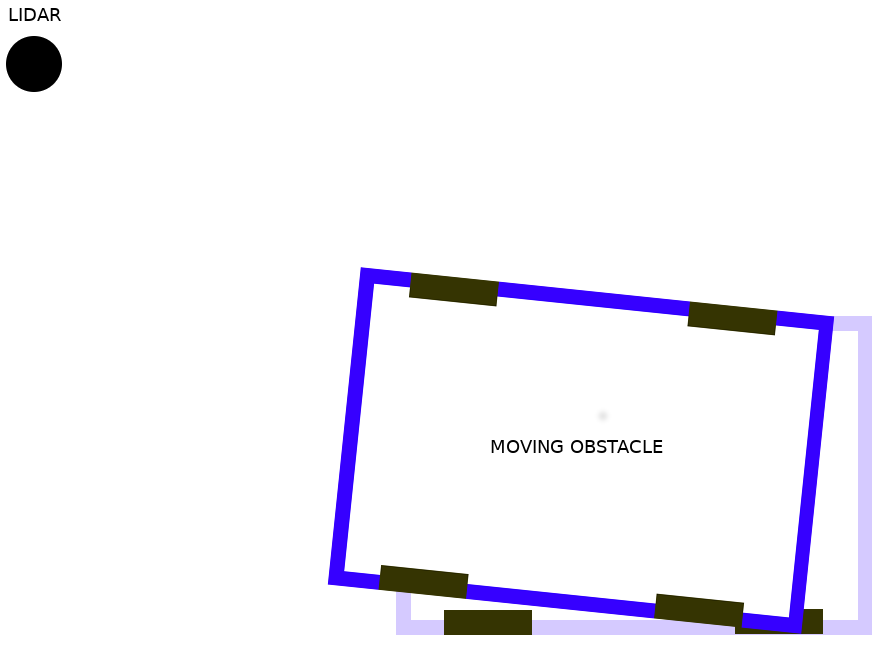
\includegraphics[height=80mm]{figures/raw/obstacle_movement.png}
    \caption{The obstacle is moving}
    \label{obstacle_movement}
\end{figure}

Figure \ref{obstacle_movement_lidar} shows how the LIDAR detects the moving object in two different timesnaps. I marked the points corresponding to the current position with red color, and the ones of the previous measurement are pale red. As it is suggested in the figure, the measurements are far from ideal, the detected points are noisy.

\begin{figure}[!ht]
    \centering
    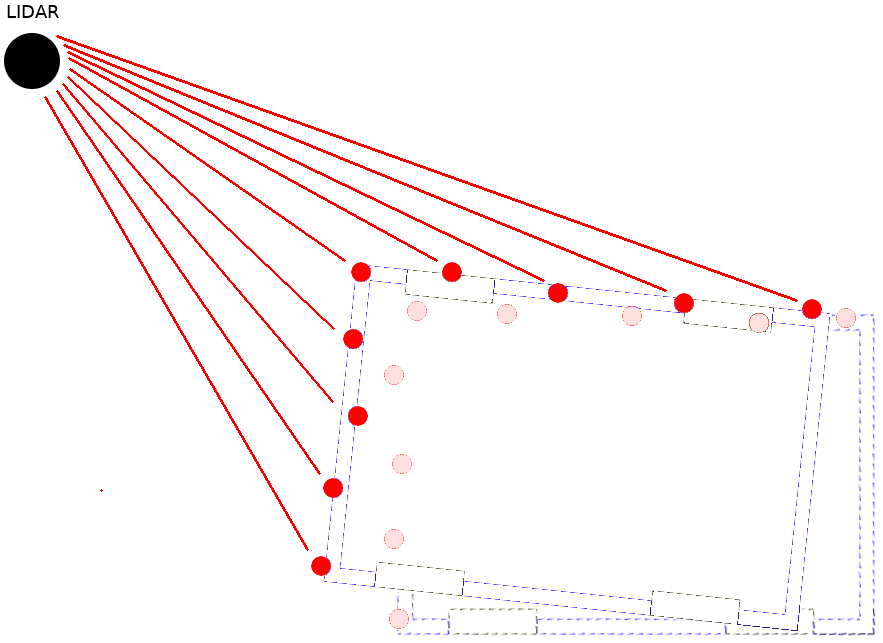
\includegraphics[height=80mm]{figures/raw/obstacle_movement_lidar.png}
    \caption{The detected points of the moving obstacle}
    \label{obstacle_movement_lidar}
\end{figure}

To understand the method of dynamic point detection, I removed the LIDAR, its virtual rays and the obstacle's contour from the image, thus leaving leaving only the measured points of the two timesnap. The result, which is basically a time-buffered array of 2D points, is presented on figure \ref{obstacle_movement_lidar_only}. The algorithm iterates through each point in the current measurement, and checks if any point in the previous measurements\footnote{The number of measurements to 'look up' is configurable.} is within its compliance radius\footnote{The compliance radius is a maximum allowed distance between measurements representing the same physical point but measured in different timesnaps. If the distance between two measurements is greater than this value, the measurements are assumed to represent different points of the space. The compliance radius is calculated for each measurement separately, and it is proportional to the distance of the LIDAR and the measured point.}.

\begin{figure}[!ht]
    \centering
    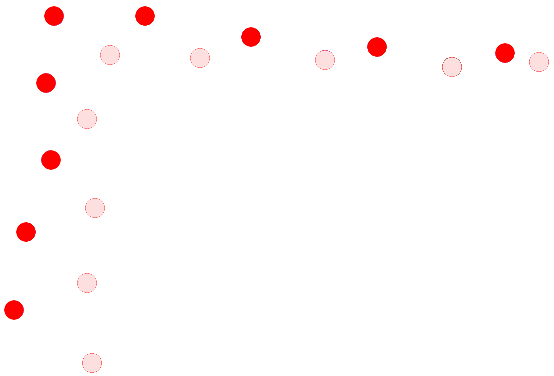
\includegraphics[height=50mm]{figures/raw/obstacle_movement_lidar_only.png}
    \caption{The detected points of the two timesnaps}
    \label{obstacle_movement_lidar_only}
\end{figure}

The measured points with their compliance radiuses are presented in \ref{compliance_radiuses}. The possible dynamic points, that have no points from the previous measurement within their radius, are marked with blue, and their compliance radius with yellow. The possible static points are marked with red, along with their radiuses. Note, that these points are \textit{possible} dynamic and static points. The final classification will be preceded be multiple filtering mechanisms and point grouping, but this is the base for finding dynamic objects.

\begin{figure}[!ht]
    \centering
    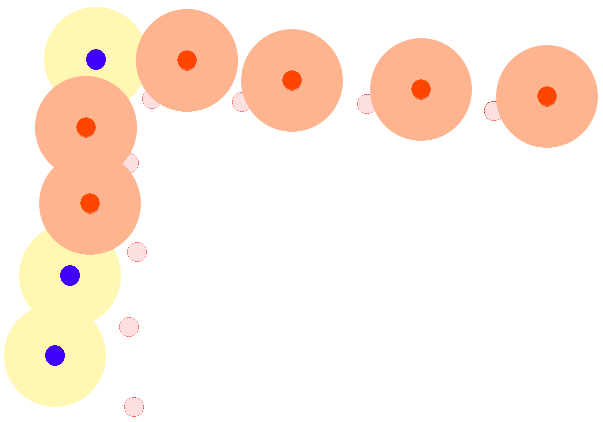
\includegraphics[height=50mm]{figures/raw/compliance_radiuses.png}
    \caption{The compliance radiuses and the dynamic points}
    \label{compliance_radiuses}
\end{figure}

Several conclusions can be drew from \ref{compliance_radiuses}. The one, and probably most important is that with right parameterizing (number of 'look-up' measurements, compliance radius, etc) this method amplifies the positive\footnote{Previously a distant background was detected, but now a closer object appears.} and negative\footnote{Previously a close object was detected, but now it disappears, and the distant background becomes visible.} changes of the scans. The second remark is that the method does not detect all the points of a moving object. However, due to measurement noise, false detections may happen, and non-moving points may be marked as dynamic.

Therefore, the result of this separation step needs to be filtered. I implemented a filtering step that only keeps those samples in the set of dynamic points, of which the left and right neighbour in the scan has also been marked dynamic. It can be easily compared to \href{https://en.wikipedia.org/wiki/Erosion_(morphology)}{erosion} in image processing, which is able to remove peaks from the image. Let's take a look at \ref{dynamic_points}. The possible dynamic points are marked with blue. The filtering mechanism iterates through each of them, and check both neighbours. As it can be easily read from the figure, point \textit{A} has two neighbours that have been marked static, therefore it will be removed from the set of dynamic points. However, points \textit{B} and \textit{C} both have dynamic neighbours (each other), so they will not be filtered out. This algorithm removes the single-size false detections from the result of the separation.

\begin{figure}[!ht]
    \centering
    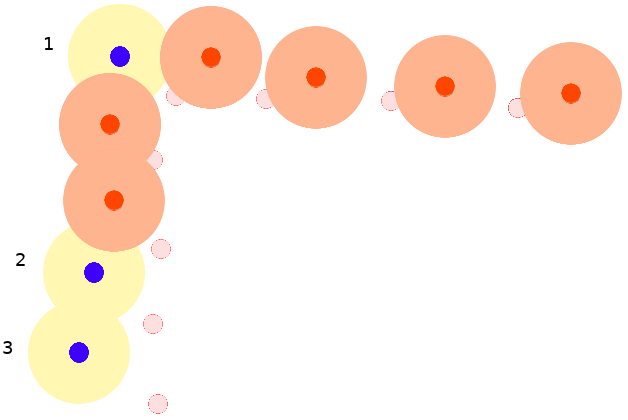
\includegraphics[height=50mm]{figures/raw/dynamic_points.png}
    \caption{Point \textit{A} will be filtered out}
    \label{dynamic_points}
\end{figure}

\subsection{Grouping}
After the filtering, we can safely assumed that the elements in the dynamic point set are in fact points of a moving obstacle. The next step is grouping the corresponding dynamic points, and also adding those points to these groups that were prevoiusly marked as static, but they are part of a moving group. For example in \ref{dynamic_points}, after the separation and filtering, only points \textit{B} and \textit{C} were marked dynamic, but actually, all the points in the image are points of the same object, that is moving. The grouping algorithm needs to be able to add these other points to the group as well.

The grouping algorithm is based on the supposition that coherent points are close to each other, while the distance between points of separate objects is larger. With a few exceptions, this statement holds its stand, by practice it proved to be a reliable base for grouping. The algorithm itself is quite simple, it separates the list of measurements (including the static and dynamic poitns as well) into subsets - groups. A new group is started when the distance between two adjacent points is larger than the permitted maximum within a group. This maximum is an empirical constant, with experiments of valid use cases. The result of the step is shown in \ref{groups}.

\begin{figure}[!ht]
    \centering
    \subfloat[Gazebo simulation]
    {
        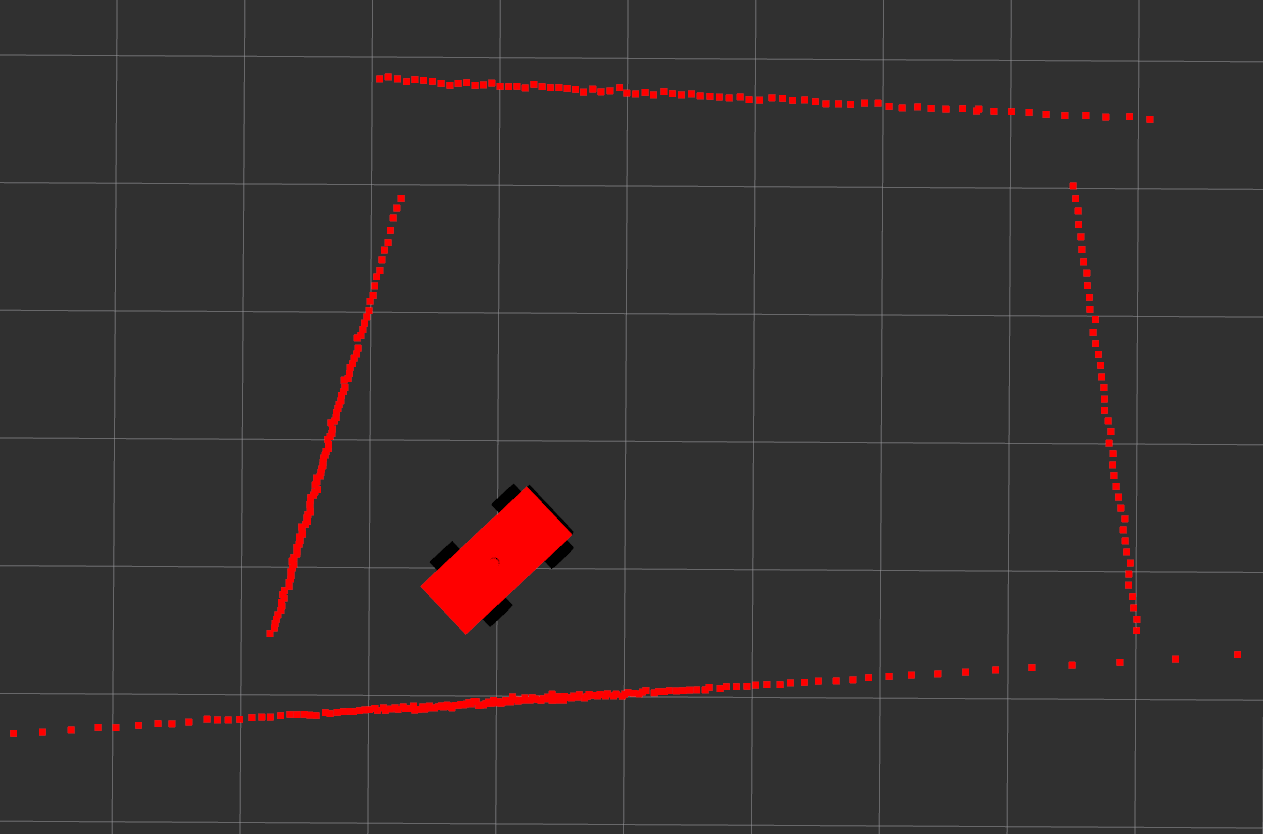
\includegraphics[height=46mm]{figures/raw/rviz_lidar_scan.png}
        \label{gazebo_wall_following_car}
    }
    \subfloat[Groups]
    {
    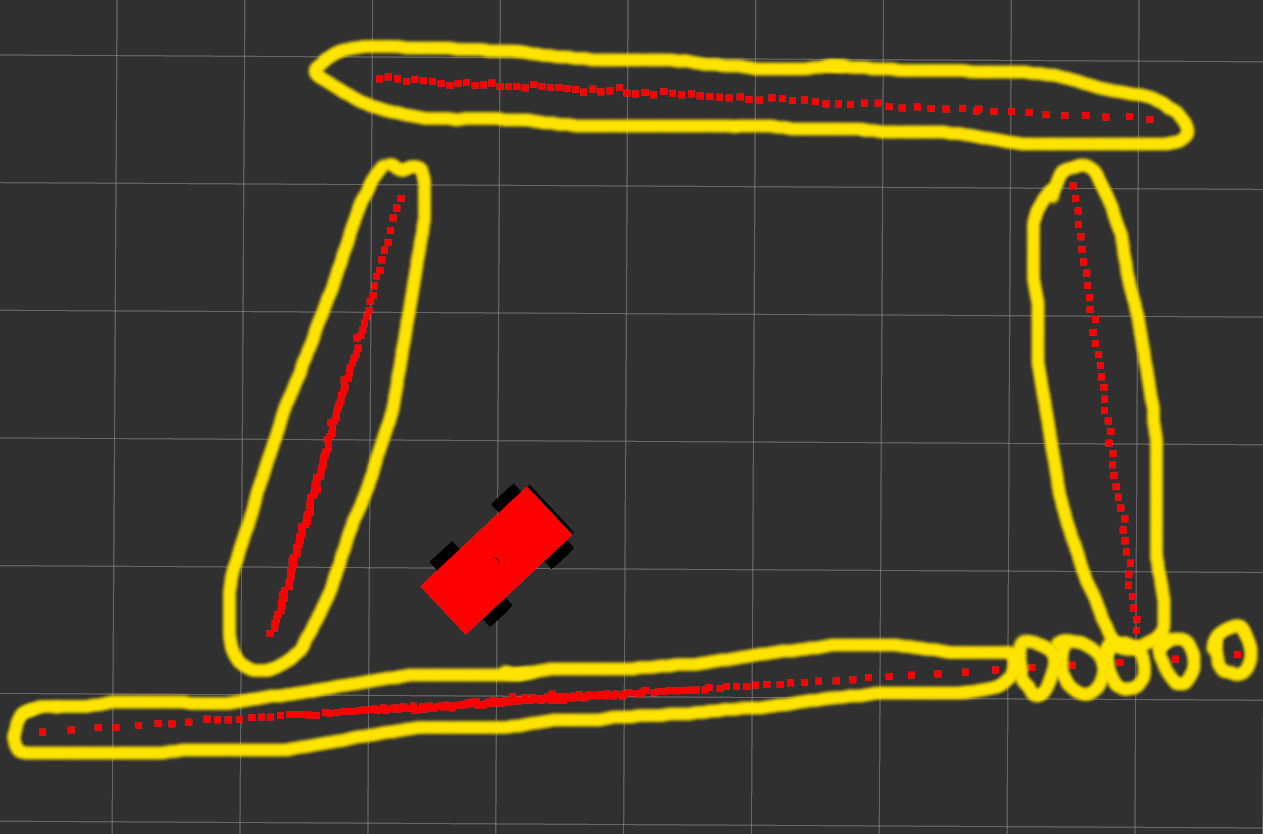
\includegraphics[height=46mm]{figures/raw/groups.png}
        \label{groups}
    }
    \caption{Distance-based grouping}
    \label{wall_following_car}
\end{figure}

As it is clearly visible on the image, far points that are correspondent to the same object may be separated from each other, and grouped one by one - see the bottom right corner of the picture. However, the further an object is from the LIDAR, the less important it is for the local trajectory planner, which needs to avoid close obstacles. But still, they are not valid groups, so as the last step of the grouping mechanism, these single-point groups will be removed from the list of groups. But before doing that, there is still one special case that needs to be handled by the grouping unit - the \textit{wall following car}. Let's imagine the situation represented in \ref{wall_following_car}. The detected obstacle (represented by the box) is moving alongside the wall, and within the maximum group point distance. Therefore, the grouping algorithm will join the groups. This wouldn't be a problem if the box wasn't moving, but as soon as it changes its position, grouping it together with the wall would ruin the mass center and speed vector calculation, described in \ref{chap:tracking}.

\begin{figure}[!ht]
    \centering
    \subfloat[Gazebo simulation]
    {
        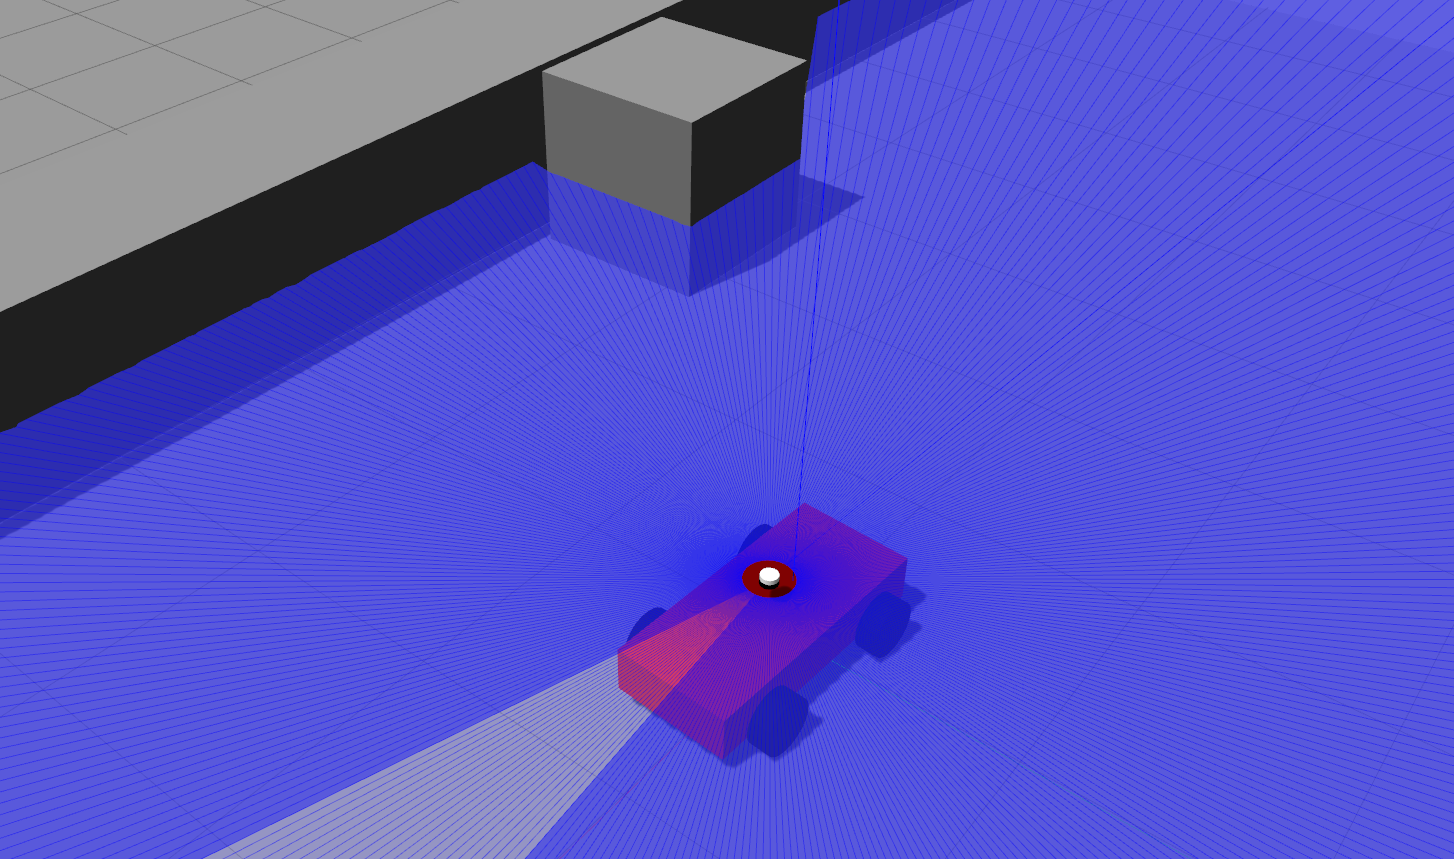
\includegraphics[height=46mm]{figures/raw/gazebo_wall_following_car.png}
        \label{gazebo_wall_following_car}
    }
    \subfloat[Lidar scan]
    {
    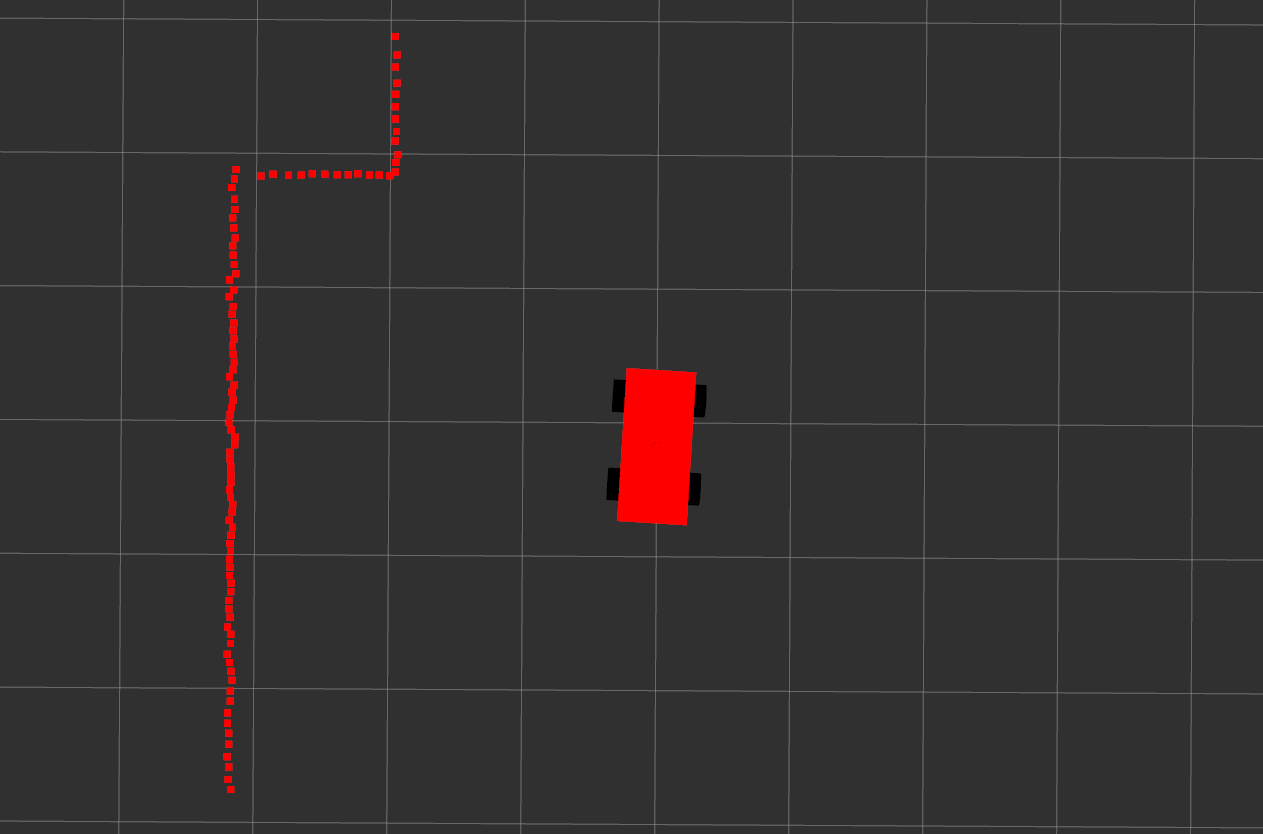
\includegraphics[height=46mm]{figures/raw/rviz_wall_following_car.png}
        \label{rviz_wall_following_car}
    }
    \caption{The \textit{wall following car}}
    \label{wall_following_car}
\end{figure}

To avoid this problem, the algorithm detects if an obstacle is unusually large, and cuts off long 'tails' from the group. Figure \ref{group_cutting} explains this step in practice.

\begin{figure}[!ht]
    \centering
    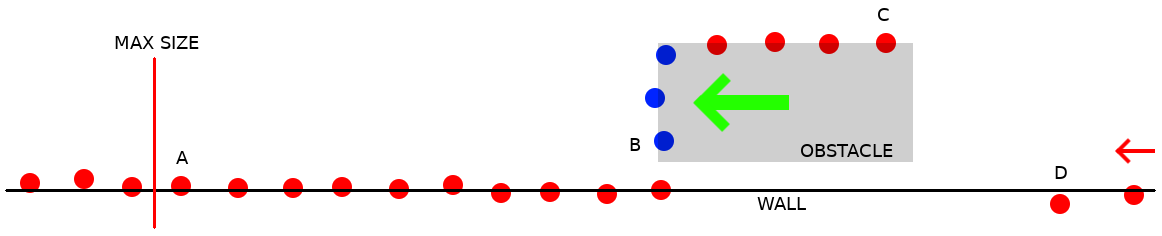
\includegraphics[width=\textwidth]{figures/raw/group_cutting.png}
    \caption{Points on the left of \textit{B} will be cut off}
    \label{group_cutting}
\end{figure}

Let's assume that the algorithm iterates through the points visualized in the figure from the right. The distance between points \textit{C} and \textit{D} is larger that the allowed maximum group point distance, therefore point \textit{C} starts a new group. Until the program reaches point \textit{A}, all the points are added to this group, because the distance between adjacent points is always lower than the maximum group point distance, but after point \textit{A}, the algorithm detects that the group is larger than the permitted limit. So the iteration turns around, and all the points are getting removed from the group, until the first dynamic point is reached - in the current example this would be point \textit{B}. As a result, only the points between (and including) point \textit{B} and point \textit{C} will be grouped together.

As an undesired side-effect, this step may also remove some of those points from the group that are in fact parts of the moving object but were marked as static, because the removal only stops at the first \textit{dynamic} point.

\subsection{Separation of static points and dynamic groups}

The previous step has successfully sorted the measured points into groups, but it is undecided yet if these groups are moving or not. This decision is made by checking the number of dynamic points in each group, which must exceed the required minimum in order to the group being marked as dynamic.

This was the last step of the separation of the groups, from this point, static points and dynamic groups will be handled differently.

\section{Dynamic obstacles}
After the dynamic groups have been separated from the static points, additional information needs to be calculated for them, so that the local track planner algorithm can use their data for its obstacle-avoidance feature. 3 pieces of information are needed for each object, its position, size and speed vector. All of these are calculated from the object's mass center, which is the average of the group points. This mass center is considered to be the object's position in space.

\begin{figure}[!ht]
    \centering
    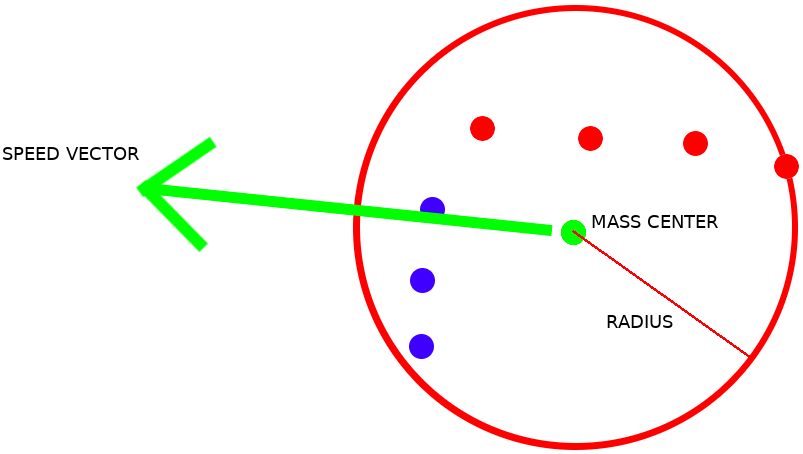
\includegraphics[height=50mm]{figures/raw/dynamic_information.png}
    \caption{The calculated information for dynamic obstacles}
    \label{dynamic_information}
\end{figure}

\subsection{Areas}
First, the groups are substituted by bounding circles. The circle's radius is the distance between the farthest group point and the mass center. This simplification results in easier path calculation in the local planner, but also drops every information known about the obstacle's shape. For long objects, for instance, this method provides a very unrealistic image of the object, because the bounding circle is much larger than the obstacle itself. But for ususal shapes such as cars, the loss that the representation causes is less than the processing time we save with the simplification.

\subsection{Tracking}
\label{chap:tracking}
Speed vectors are calculated from the change of the mass center between measurements. But in order to be able to check the mass center of a group in any previous measurement, object tracking is needed. The tracking is done by estimating each obstacles' current position based on their previous positions and speed vectors, and finding the best fit among the current groups. Filtering is also needed for such false detections when a previously detected object is not recognized for a few cycles. Without filtering, these obstacles would disappear from the list of groups for a period of time and then they would reappear, but tracking would fail. Therefore the algorithm keeps these objects alive for a given number of measurement periods, updating their positions with their last known speed vector in every cycle.

\begin{figure}[!ht]
    \centering
    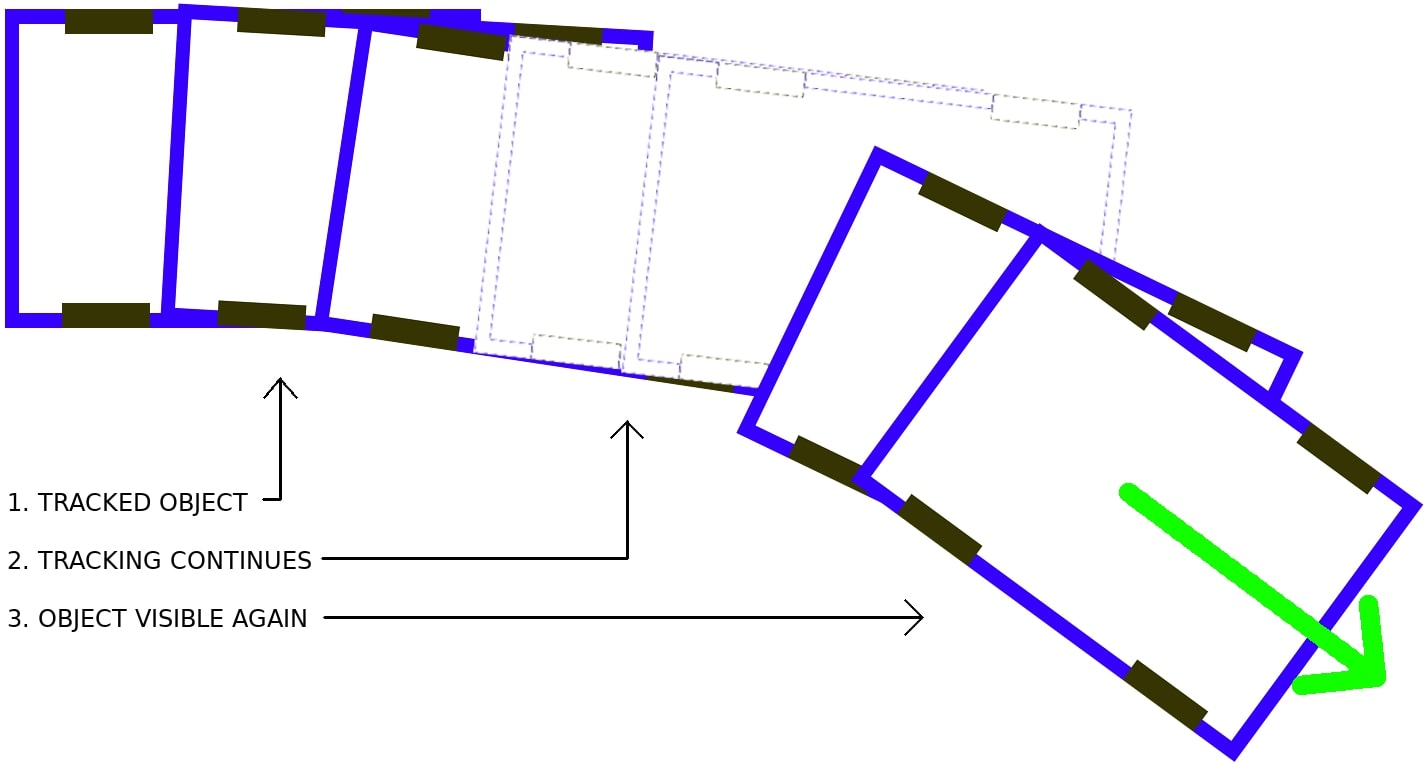
\includegraphics[width=\textwidth]{figures/raw/tracking.png}
    \caption{Object tracking}
    \label{tracking}
\end{figure}

After the objects have been tracked, their speed vectors can be calculated. A filter is applied here, as well, for smoother obstacle paths.

\subsection{Publishing dynamic obstacles}
\label{chap:publishing_dynamic_obstacles}
Dynamic obstacles - as outputs of the mapping node - are published on several topics, responsible for containing information for further processing. The array of dynamic objects is published on the \textit{dynamic\_objects} topic of type \textit{environment\_builder/DynamicObjectArray} (an array of \textit{environment\_builder/DynamicObject}s, which is a custom type for representing the detected obstacles in the map. It's format is the following:

\begin{minipage}{\textwidth}
\begin{lstlisting}[language=IDL]
float32 radius
geometry_msgs/Pose pose
geometry_msgs/Twist twist
\end{lstlisting}
\end{minipage}

And the structure of \textit{environment\_builder/DynamicObjectArray} is simply:

\begin{lstlisting}[language=IDL]
DynamicObject[] objects
\end{lstlisting}

The node also publishes messages that are useful for visualization and diagnostics or debugging. On topic \textit{obstacles}, visualization messages of type \href{http://docs.ros.org/melodic/api/visualization_msgs/html/msg/MarkerArray.html}{\textit{visualization\_msgs::MarkerArray}} are published. This type of message contains an array of \href{http://docs.ros.org/melodic/api/visualization_msgs/html/msg/Marker.html}{\textit{visualization\_msgs::Marker}}s, which look like the following:

\begin{minipage}{\textwidth}
\begin{lstlisting}[language=IDL]
uint8 ARROW=0
uint8 CUBE=1
uint8 SPHERE=2
uint8 CYLINDER=3
uint8 LINE_STRIP=4
uint8 LINE_LIST=5
uint8 CUBE_LIST=6
uint8 SPHERE_LIST=7
uint8 POINTS=8
uint8 TEXT_VIEW_FACING=9
uint8 MESH_RESOURCE=10
uint8 TRIANGLE_LIST=11
uint8 ADD=0
uint8 MODIFY=0
uint8 DELETE=2
uint8 DELETEALL=3
std_msgs/Header header
string ns
int32 id
int32 type
int32 action
geometry_msgs/Pose pose
geometry_msgs/Vector3 scale
std_msgs/ColorRGBA color
duration lifetime
bool frame_locked
geometry_msgs/Point[] points
std_msgs/ColorRGBA[] colors
string text
string mesh_resource
bool mesh_use_embedded_materials
\end{lstlisting}
\end{minipage}

With its \textit{type} set to either \textit{SPHERE} or \textit{ARROW}, these markers represent the areas and speed vectors of the objects, and are easily visualizable in rviz.

\begin{figure}[!ht]
    \centering
    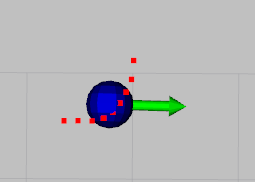
\includegraphics[height=50mm]{figures/raw/rviz_moving_object.png}
    \caption{Visualizing moving objects}
    \label{rviz_moving_object}
\end{figure}

And on topic \textit{diff\_grid}, \href{http://docs.ros.org/melodic/api/nav_msgs/html/msg/OccupancyGrid.html}{\textit{nav\_msgs/OccupancyGrid}}s are published. This is topic is purely for diagnostic and debugging purposes. It represents the dynamics of the map compared to the previous measurement, using an occupancy grid. This means that the occupancy grid will have high values where something changed in the map, an will store low values where the map is still. The algorithm that searches for dynamic objects uses this grid as its basis. The structure of the message is as follows:

\begin{minipage}{\textwidth}
\begin{lstlisting}[language=IDL]
std_msgs/Header header
nav_msgs/MapMetaData info
int8[] data
\end{lstlisting}
\end{minipage}

Where \textit{data} stores the actual grid values and \textit{info} is a \href{http://docs.ros.org/melodic/api/nav_msgs/html/msg/MapMetaData.html}{\textit{nav\_msgs/MapMetaData}}, storing meta information about the grid:

\begin{minipage}{\textwidth}
\begin{lstlisting}[language=IDL]
time map_load_time
float32 resolution
uint32 width
uint32 height
geometry_msgs/Pose origin
\end{lstlisting}
\end{minipage}

\section{Static points}
Static points used for two separate purposes. The first one is building a static map, the second is localization with the help of gmapping.

\subsection{Static map}
\label{chap:static_map}
After separating the dynamic groups from the scan points, only the static points are left. These points do not change their positions with time\footnote{Except those obstacles that start moving only after they have already been detected as sets of static points. But these objects do not ruin the quality of the map, either.}, so they can be added to the static map.

For static map-building, gmapping has already been mentioned as a candidate, but unfortunately, its algorithm does not recognize changes in the environment. In practice, if an object has been detected and placed in its map, it will not be erased from there, even after the object has moved away. Figures \ref{gmapping_drawback_before_move} and \ref{gmapping_drawback_after_move} demonstrate the problem.

\begin{figure}[!ht]
    \centering
    \subfloat[Gazebo simulation]
    {
        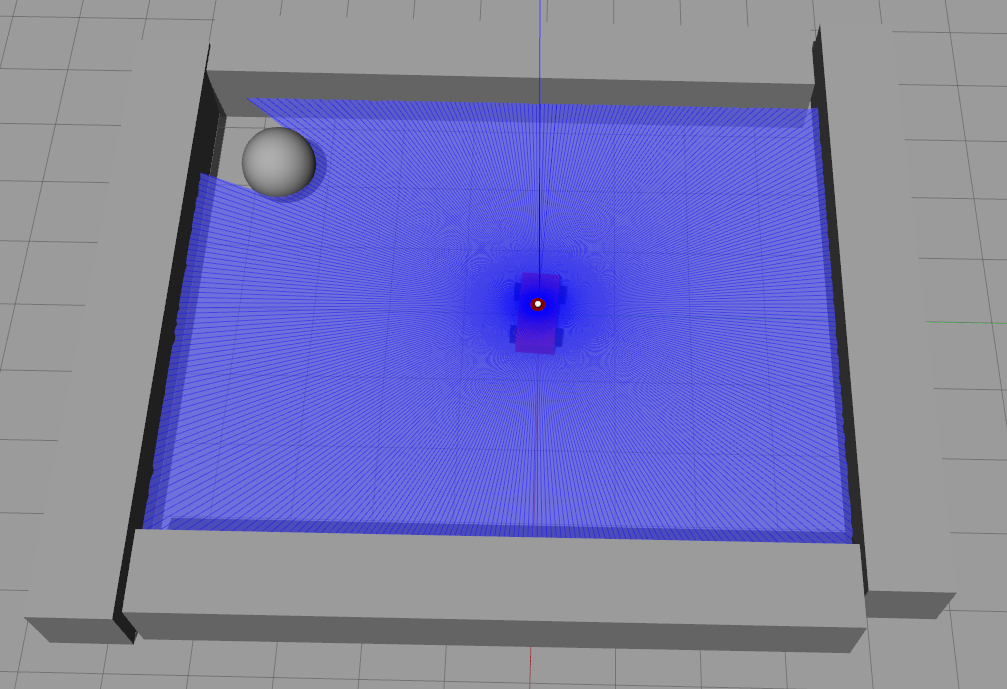
\includegraphics[height=48mm]{figures/raw/gazebo_gmapping_before_move.png}
        \label{gazebo_gmapping_before_move}
    }
    \subfloat[Map created by gmapping]
    {
    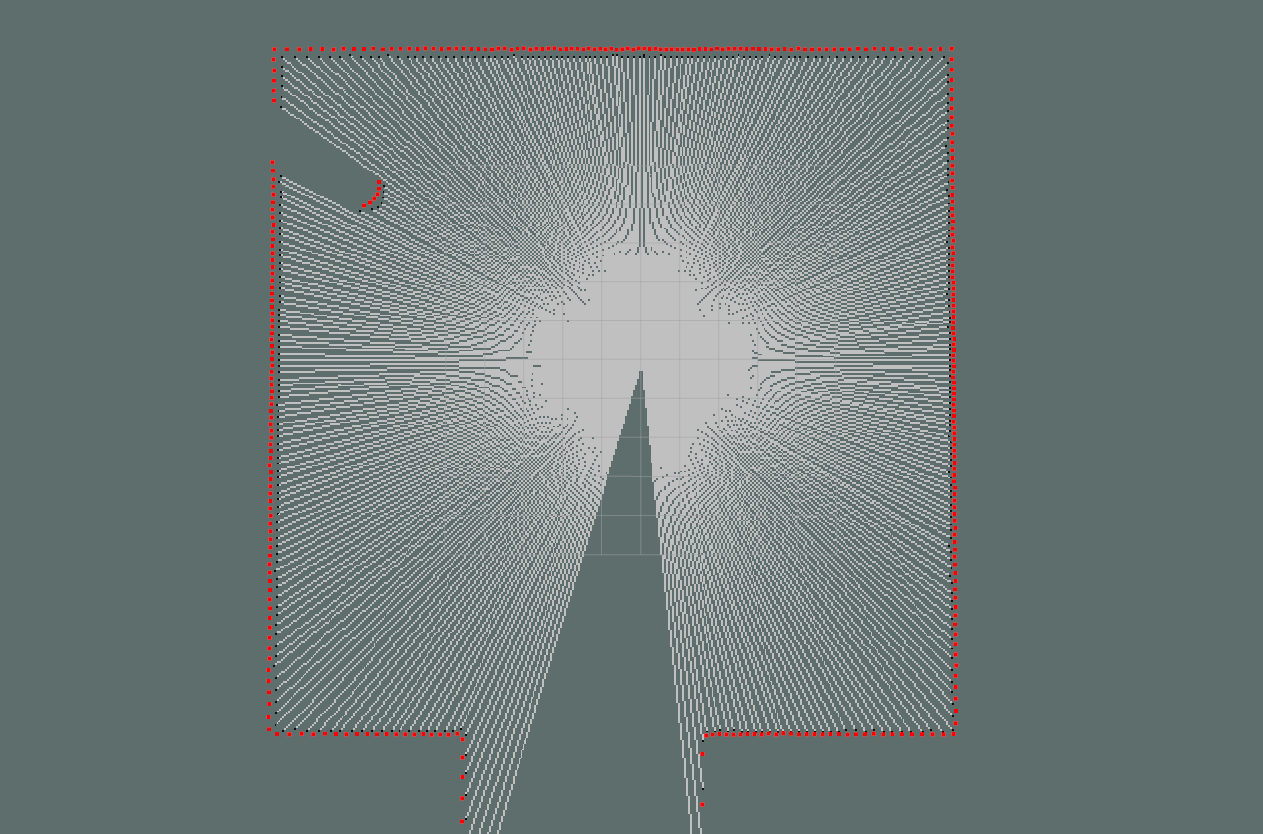
\includegraphics[height=48mm]{figures/raw/rviz_gmapping_before_move.png}
        \label{rviz_gmapping_before_move}
    }
    \caption{Initial state - ball is still}
    \label{gmapping_drawback_before_move}
\end{figure}

\ref{gmapping_drawback_before_move} shows a situation where the ball is standing still. The mapping algorithm of gmapping successfully creates a map (in the form of an occupancy grid\footnote{An occupancy grid represents a map in an evenly spaced field of probability values representing if the grid points are occupied by an obstacle}) that marks the place of the ball as occupied. However, when the ball starts moving (see \ref{gmapping_drawback_after_move}), the map does not change, because the algorithm cannot handle moving obstacles.

\begin{figure}[!ht]
    \centering
    \subfloat[Gazebo simulation]
    {
        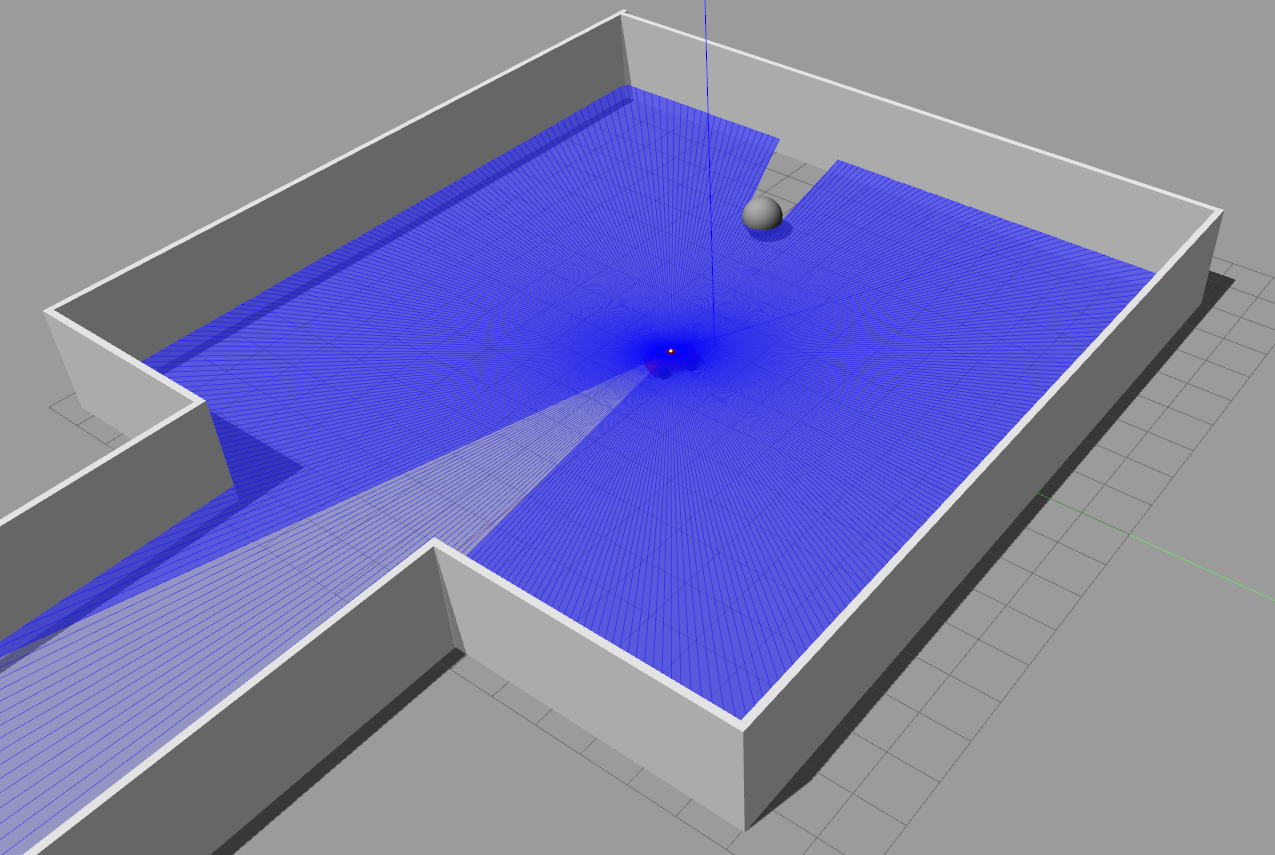
\includegraphics[height=48mm]{figures/raw/gazebo_gmapping_after_move.png}
        \label{gazebo_gmapping_after_move}
    }
    \subfloat[Map created by gmapping]
    {
        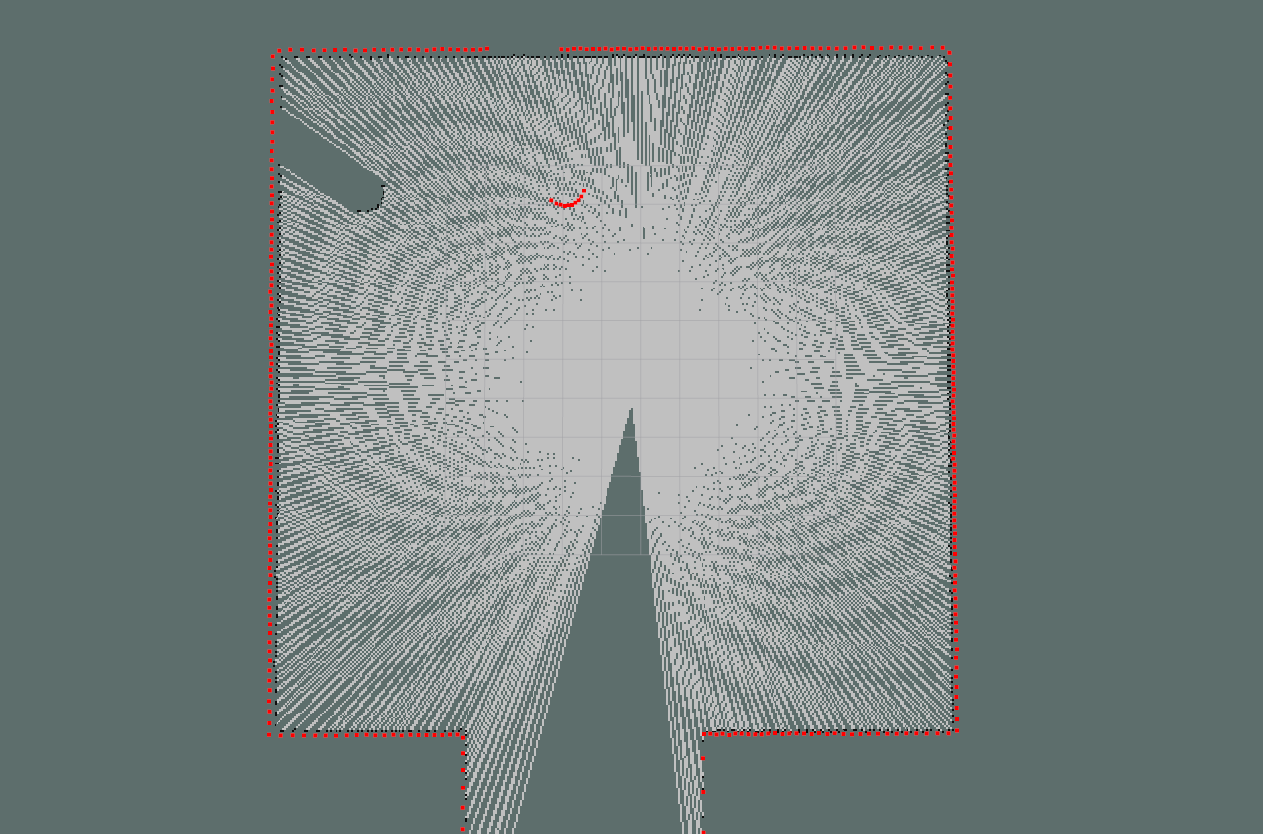
\includegraphics[height=48mm]{figures/raw/rviz_gmapping_after_move.png}
        \label{rviz_gmapping_after_move}
    }
    \caption{Moving state - ball has changed position}
    \label{gmapping_drawback_after_move}
\end{figure}

Due to the above problem, static map-building needed to be implemented internally, which is basically a 2D occupancy grid. The grid points' possible values are the following:

\begin{center}
    \begin{tabular}{ c c }
        
\includegraphics[height=3mm]{figures/raw/map_occupied.png} & Occupied (value: 100) \\
        
\includegraphics[height=3mm]{figures/raw/map_unknown.png}  & Unknown (value: 50)   \\
        
\includegraphics[height=3mm]{figures/raw/map_free.png}     & Free (value: 0)       \\
    \end{tabular}
\end{center}

I chose the most straight-forward way of map-building - each static measurement introduces an occupied point and a free ray in the map. The map's size and resolution can be set as input parameters (see MAP\_SIZE and MAP\_RES in \ref{chap:input_parameters}). \ref{map_ray} visualizes the situation. The green and red grids are the car's current position and the measured point.

\begin{figure}[!ht]
    \centering
    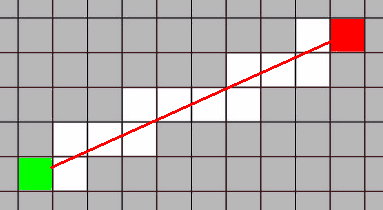
\includegraphics[height=50mm]{figures/raw/map_ray.png}
    \caption{Introducing a free ray}
    \label{map_ray}
\end{figure}

\subsection{Publishing static points}
\label{chap:publishing_static_points}
The built static map is published on topic \textit{static\_grid}, which is a \href{http://docs.ros.org/melodic/api/nav_msgs/html/msg/OccupancyGrid.html}{nav\_msgs/OccupancyGrid}, just like the previously introduced \textit{diff\_grid} topic's messages.

With the publishing of the maps the mapping node has finished its task, and the focus now shifts to the motion planning node which calculates actuations that drive the car to the destination without hitting any static or dynamic objects.